\documentclass{beamer}
% AnnArbor  Antibes  Bergen  Berkeley  Berlin  Boadilla  CambridgeUS  Copenhagen  Darmstadt  Dresden  Frankfurt  Goettingen  Hannover  Ilmenau  JuanLesPins  Luebeck  Madrid  Malmoe  Marburg  Montpellier  PaloAlto  Pittsburgh  Rochester  Singapore  Szeged  Warsaw  boxes  default 
\mode<presentation>
    {
      \usetheme{Berkeley}
      \setbeamercovered{transparent}
    }
    \usepackage[english]{babel}
    \usepackage{graphicx}           
    \usepackage{xeCJK}       
    \usepackage{fontspec}
    \usepackage{courier}
    
    \title[A Case Study in SoF] {A Case Study in Stakeholder-oriented Goal-modeling Framework}
          
    \subtitle{}
              
    \author[Author]{Jipeng Wu \and Eryu Ding \and Bin Luo}
                     
     \institute[Universities of Somewhere and Elsewhere] {
                                 Software Institute\\
                                 Nanjing University
     }
                               
\date[ICSESS 2014]
{ICSESS Presentations, 2014}

\subject{Theoretical Computer Science}
\AtBeginSubsection[]
{
  \begin{frame}<beamer>{Outline}
    \tableofcontents[currentsection,currentsubsection]
  \end{frame}
}

%10~12 minutes oral presentation
\begin{document}

\begin{frame}
  \titlepage
\end{frame}

\begin{frame}{Outline}
  \tableofcontents
\end{frame}

\section{Motivation}
\subsection{The Basic Problem That We Studied}
\begin{frame}{Why We Presented SoF}              %[1]
  \begin{itemize}
  \item
    We applied goal methods in a RE process. To guide a RE process, we presented a possible solution——SoF(Stakeholder-oriented Goal Modeling Framework).
    \begin{itemize}
    \item Goal methods
      %includes: goal modeling, goal specification, goal analysis(formal or informal, validation, verification, elaboration, conflict management)
      %We do need these methods, they are the core of goal-based RE, but they are not enough to compose a complete RE process.
      %RE process, more precisely speaking, the early phase of RE process is our research target.
      \begin{itemize}
      \item diverse, but discrete and fragmental  
      \item rely on a certain context 
      \end{itemize}
    \item RE process 
      \begin{itemize}
      \item consistent and monolithic 
      \item not reply on a certain context.   Because it is context itself.
      \end{itemize}
    \end{itemize}
  \end{itemize}
\end{frame}
\begin{frame}{Why We Presented SoF}          %[2]
  \begin{itemize}
  \item We do need these methods, they are the core of goal-based RE, but they are not enough to compose a complete RE process
  \item 
    On the abstraction level of RE process, the most important RE concerns are: 
    \begin{itemize}
    \item a general workflow and details of each step 
    \item how to build models and other RE artefacts 
    \item a way to obtain initial goals 
    \item a mechanism to ensure correctness of goal-reasoning results 
    \end{itemize}
  \end{itemize}
\end{frame}

\begin{frame}{Features of SoF}             %[3]
  \begin{itemize}
  \item Goals acquition 
    \begin{enumerate}
    \item scenario-based interviews with stakeholders 
    \item a structured scenario description to organize the interview results 
    \end{enumerate}
  \item Goal modeling  
    \begin{enumerate}
    \item a KAOS-like top-down decomposed goal tree model  
    \item goal models with RWS-style annotations for stakeholder validation. 
    \end{enumerate}
  \item Atomicity of some Processes 
    \begin{enumerate}
    \item Acquition, elaboration and validation of the same goal are non-interruptible processes. 
    \item During an atomic activity, the goal is inaccessible. 
    \item Input goals of an atomic activity should be output goals of another atomic activity or initial goals.
    \item Thus the correctness of each single atomic activity ensures the correctness of the whole goal reasoning process.
    \end{enumerate}
  \end{itemize}
\end{frame}


\subsection{Previous Work}             %[4]
\begin{frame}{KAOS Goal Model}
  \begin{itemize}
  \item
    KAOS [van Lamsweerde, 1995]
    \begin{enumerate}
    \item
      Although KAOS is a complete RE approach, we are concerned only with its goal model. 
    \item
      KAOS goal model defines some meta-concepts—goal, action, agent, entity and event, which can be visualized as nodes.
    \item 
      The edges between nodes capture the semantic links between such abstractions.
      \begin{enumerate}
      \item Two basic link types——AND/OR.
      \item Extended link types: Contributes(+), ContributesStrongly(++), Conflicts(-), and ConflictsStrongly(--).
      \end{enumerate}
    \end{enumerate}
  \end{itemize}
\end{frame}
\begin{frame}{Real World Scene Annotation}                     %[5]
  \begin{itemize}
  \item
    Real World Scenes [Haumer, 1998]  % a scenario-based approach
    \begin{enumerate}
    \item
      Current system should be captured in the form of rich media(e.g., taking photos, recording videos). The observation results are called Real World Scene. 
    \item 
      The observation results should be linked to goals, in order to elaborate and validate goals in the follow-up work.
    \item
      RWS annotated the goal model with views of stakeholders(1.agree, 2.not agree, 3.add more goals and 4.no position), which facilitates review and validation and finally conforms the goal model to the real world scene. 
    \end{enumerate}
  \end{itemize}
\end{frame}

\section{Our Proposal and Case Study}
\subsection{SoF Process}

\begin{frame}{SoF Elaboration Activity}
  \begin{enumerate}
  \item
    SoF combines requirements acquition, requirements elaboration reasoning and requirements validation as one atomic activity, which is called \emph{SoF Elaboration Activity}.
  \item
    Each successful \emph{SoF Elaboration Activity} includes the following phases: 
    \begin{enumerate}
    \item interviews with stakeholders, updating \emph{"Scenario Description"}
    \item elaborating goal models % using KAOS methods
    \item validation interview
    \end{enumerate}
  \item
    Before all the steps of the \emph{SoF Elaboration Activity} of one requirement have been finished, it is not allowed that the \emph{SoF Elaboration Activity} of another requirement is initiated. 
  \end{enumerate}
\end{frame}

\begin{frame}{Activity Diagram of SoF Process}
  \begin{figure}
    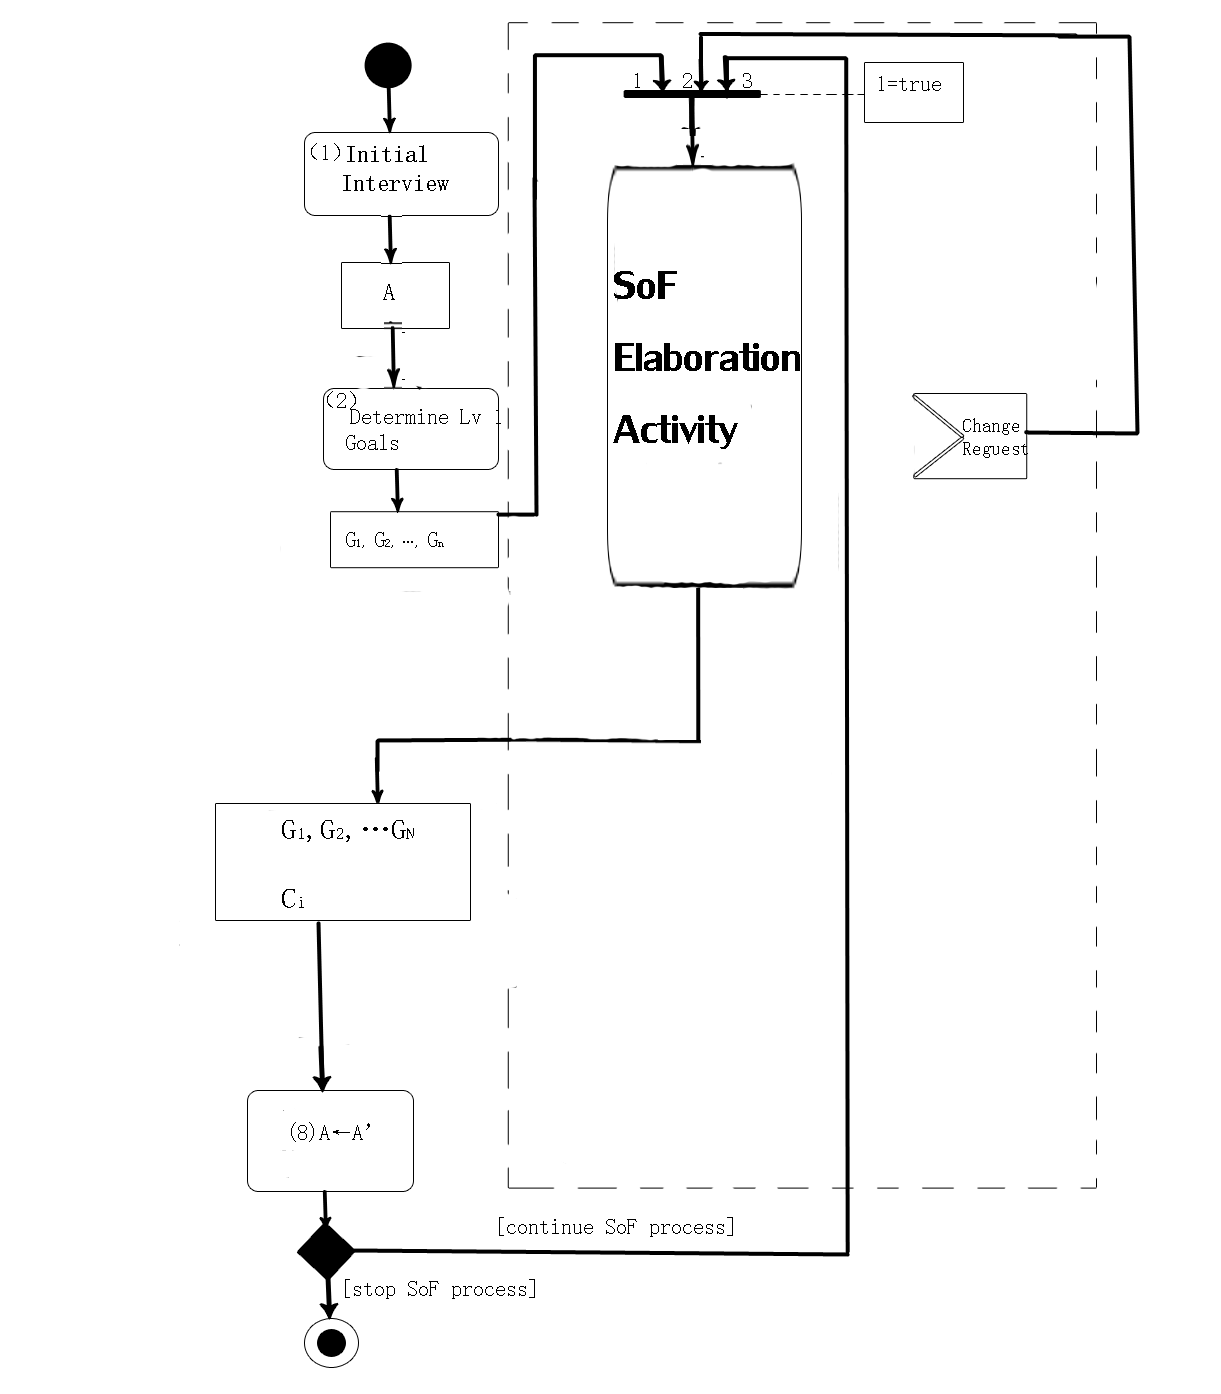
\includegraphics[width=2.4in]{img/2_0.PNG}
    \caption{Activity Diagram of SoF Process}
  \end{figure}
\end{frame}  

\begin{frame}{Detailed Activity Diagram of SoF Process}
  \begin{figure}
    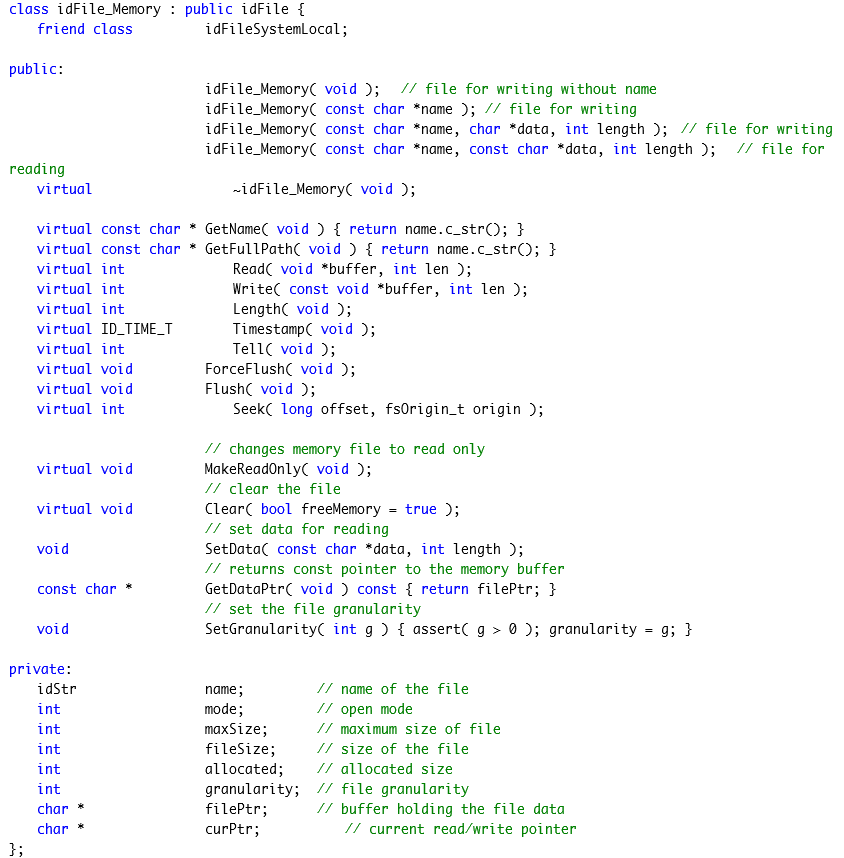
\includegraphics[width=2.4in]{img/2.PNG}
    \caption{Activity Diagram of SoF Process}
  \end{figure}
\end{frame}

\begin{frame}{Detailed Activity Diagram of SoF Process}
  \begin{figure}
    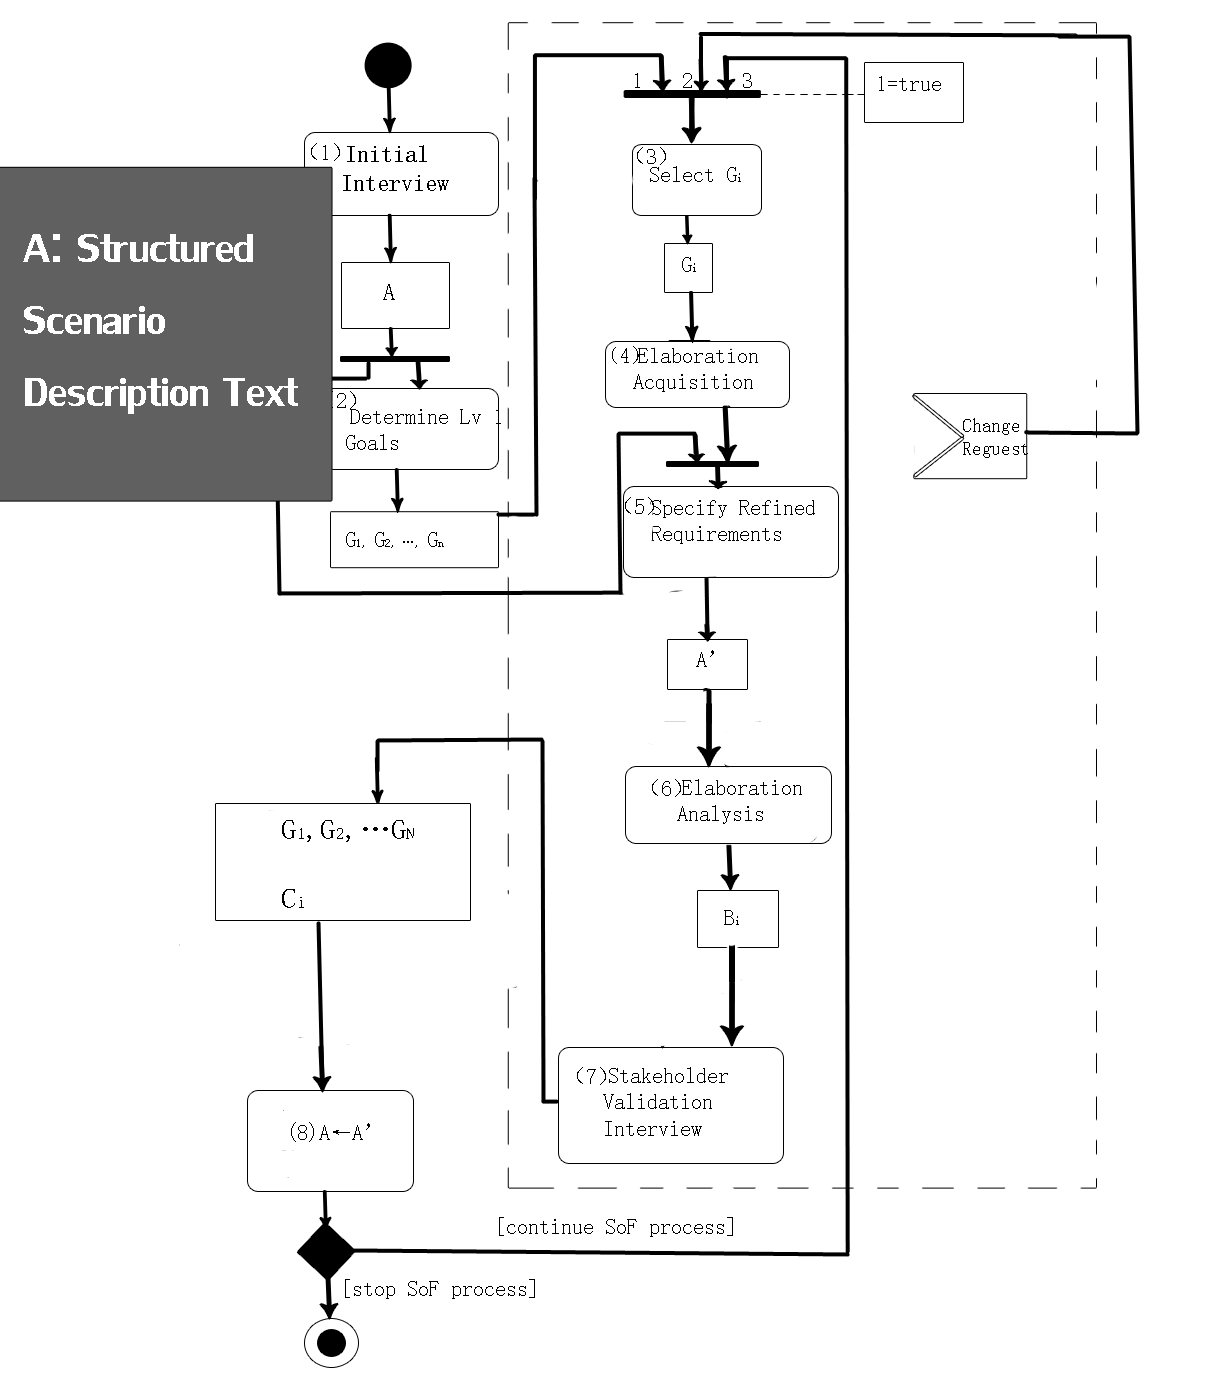
\includegraphics[width=2.4in]{img/2_1.PNG}
    \caption{Activity Diagram of SoF Process}
  \end{figure}
  %The first initial interview generates a brief structured specification, describing initial goals in the form of scenarios. This specification is updated after requirements acquisition phase of each \emph{SoF Elaboration Activity}. Each update is a basis of subsequent goal refinement and goal validation.
\end{frame}

\begin{frame}{Detailed Activity Diagram of SoF Process}
  \begin{figure}
    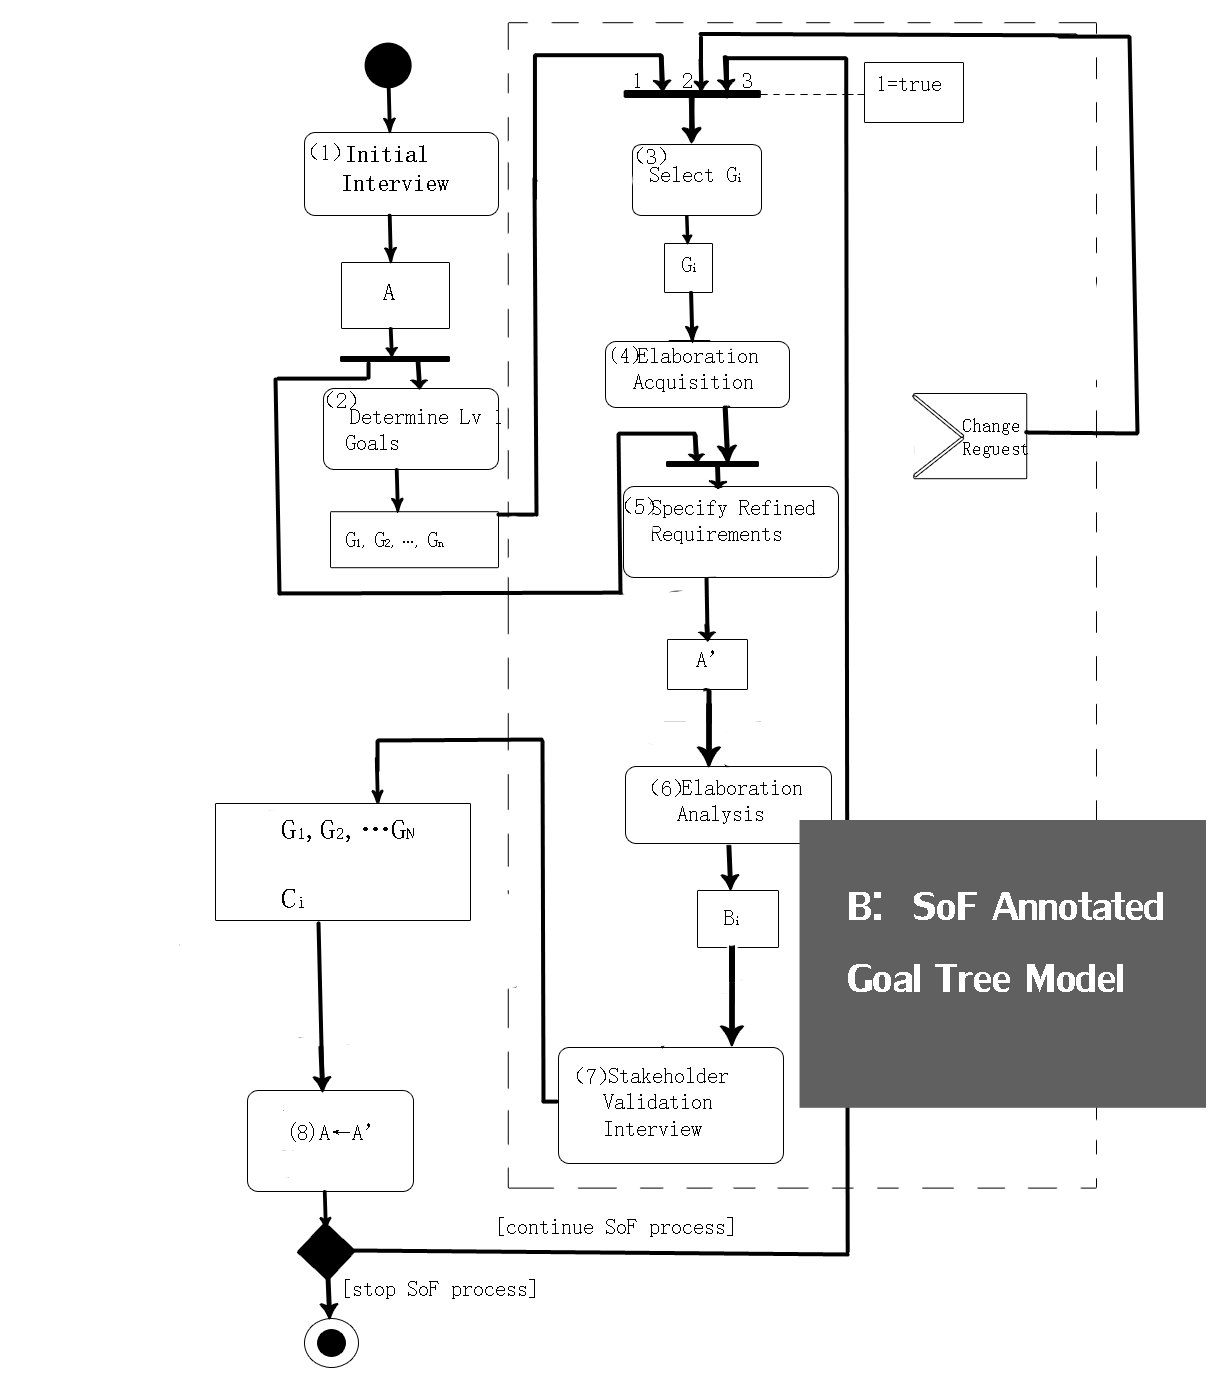
\includegraphics[width=2.4in]{img/2_2.PNG}
    \caption{Activity Diagram of SoF Process}
  \end{figure}
  %The goal model is further elaborated after each "SoF Elaboration Activity".
\end{frame}  


\subsection{Structured Scenario Description}
\begin{frame}{Why is a Scenario Description Needed?}
  \begin{itemize}
  \item
    A summary of stakeholder interview.  It records stakeholders' expectations of the future system.
  \item
    A readable document for stakeholders.   Scenarios are used to organize complex requirements.  
  \item
    A basis of subsequent goal refinement and goal validation. 
  \end{itemize}
\end{frame}

\begin{frame}{How to Build a Scenario Description?}
  \begin{itemize}
  \item
    Design goal acquition interview and prepare scenario-based questions.
  \item
    Documentation of knowledge acquired from stakeholders.
  \item
    Unlimited ways to write a scenario description. 
    \begin{enumerate}
    \item Formal or Informal   
    \item In Nature Language or Algebraic Language.
    \item Flat text or specific data structure.
    \end{enumerate}
  \end{itemize}
\end{frame}


\begin{frame}{Example of a Possible Implementation of Scenario Description}
  \begin{figure}
    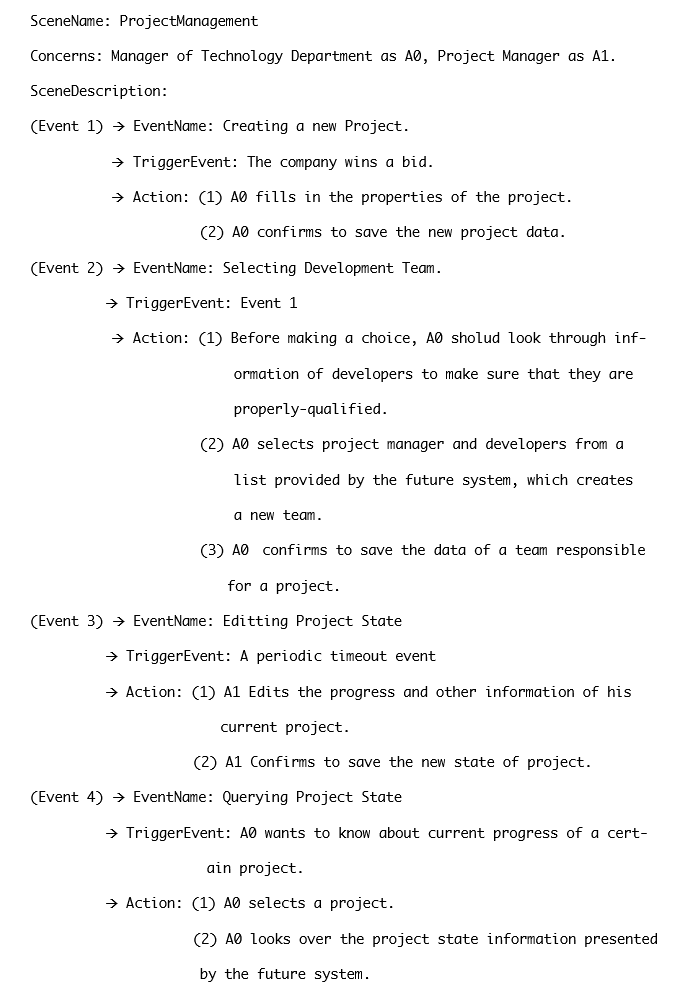
\includegraphics[width=2.0in]{img/3.PNG}
    \caption{Structured Scenario Description In Nature Language}
  \end{figure}
\end{frame}  

\begin{frame}{Example of a Possible Implementation of Scenario Description}
  \begin{enumerate}
  \item
    In this example, stakeholders describe the scenario: "how a technical manager manage projects." 
  \item 
    This scenario includes four events: 
    \begin{enumerate}
    \item \emph{create a project}
    \item \emph{select development team}
    \item \emph{edit project info}
    \item \emph{and query project progress}
    \end{enumerate}
  \item Informal but Informative 
    \begin{enumerate}
    \item It used in goal validation interviews because its readability. 
    \item Goal elaboration should not directly use this informal description, but the information provided by it helps the reasoning of \emph{SoF Annotated Goal Tree Model}.
    \end{enumerate}
  \end{enumerate}
\end{frame}  


\subsection{SoF Annotated Goal Tree}
\begin{frame}{Design of Annotated Goal Tree Model}
  \begin{enumerate}
  \item Modeling:
    \begin{enumerate}
    \item KAOS Goal Model  (top-down decomposed)
    \item RWS Annotation  (for stakeholder validation)
    \end{enumerate}
  \item A goal reasoning tool: 
    \begin{enumerate}
    \item Goal Refinement Reasoning
    \item Goal Confict Management
    \item Requirements Evaluation
    \end{enumerate}
  \item A documentation of goals
  \item A communication material in validation interviews
  \end{enumerate}
  %The annotations can be used to organize more structured evaluation interviews and actively engage stakeholders in such interviews.
  %After high-level goals determined in an initial interview, the subsequent activities, such as goal elicitation, conflict resolution and requirements evaluation, will be executed based on \emph{SoF Annotated Goal Tree Model}.
\end{frame}  
\begin{frame}{2 types of Goal Elaboration Results}
  \begin{enumerate}
  \item Pass: a basis of the next \emph{SoF Elaboration Activity} 
  \item Failure: a driven model for communication with stakeholders and control of requirements changes. 
  \item Goal validation phase of \emph{SoF Elaboration Activity} can be further decomposed according to the design of annotations of \emph{SoF Annotated Goal Tree Model}.
    \begin{enumerate}
    \item relevance validation
    \item success validation
    \end{enumerate}
  \end{enumerate}
\end{frame}

\begin{frame}{\emph{SoF Annotated Goal Tree Model} adds the following two types of marks:}            
  \begin{itemize}
  \item
    The mark "relevance" is used to record whether a goal has passed relevance validation.
%    The evaluation is based on stakeholders perspectives and latest structured specification based on scenarios.
%    If the goal is irrelevant to the future system, it is marked with No, otherwise it is marked with Yes.
%    Goals cannot enter the next step of success validation until it passes the relevance validation.
  \item
    The mark "agreed" is used to record whether a relevant goal has passed success validation.
%    The evaluation is based on stakeholders perspectives on the practical significance, constraints and cost of the evaluated goal. If a it does not agree with stakeholders' expectations, the goal should be still denied.
  \end{itemize}
\end{frame}


%\begin{frame}  {Goal Elaboration-->Image!!}
%  \begin{itemize}
%    \begin{enumerate}
%    \item  In Fig.3 we present a high-level goal $G_1$—"To make technical department manager make better decisions when build project teams".
%    \item  By asking Why/How questions we get child goals supporting $G_1$: $G_{1.1}$ and $G_{1.2}$.
%      \begin{enumerate}
%      \item  $G_{1.1}$ is "To provide better support of information on developers and project managers for techinical department manager".
%      \item  $G_{1.2}$ is "To provide a mechanism allowing developers to reply with feedback to the manager's decisions".
%      \end{enumerate}
%    \item  These two goals were validated as child goals supporting their parent goal in different aspects, and thus successfully passed relevance validation. Stakeholders agreed that these two goals are consistent with their expectations. The goal tree was allowed to be further refined after each goal had passed both validations.
%    \end{enumerate}
%  \end{itemize}
%\end{frame}

\begin{frame}  {Goal Elaboration}
  \begin{figure}
    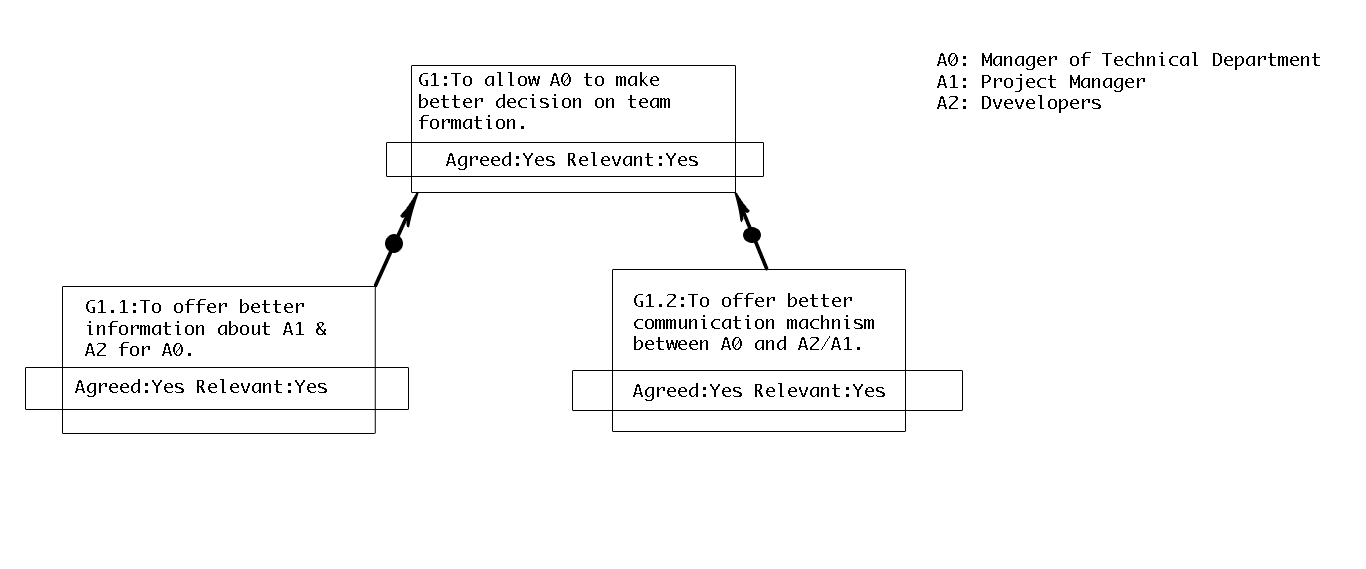
\includegraphics[width=3.4in]{img/4.PNG}
    \caption{SoF Annotated Goal Tree(Validated,Level 1 Elaboration)}
  \end{figure}
\end{frame}

\begin{frame} {Further Elaboration}
  \begin{figure}
    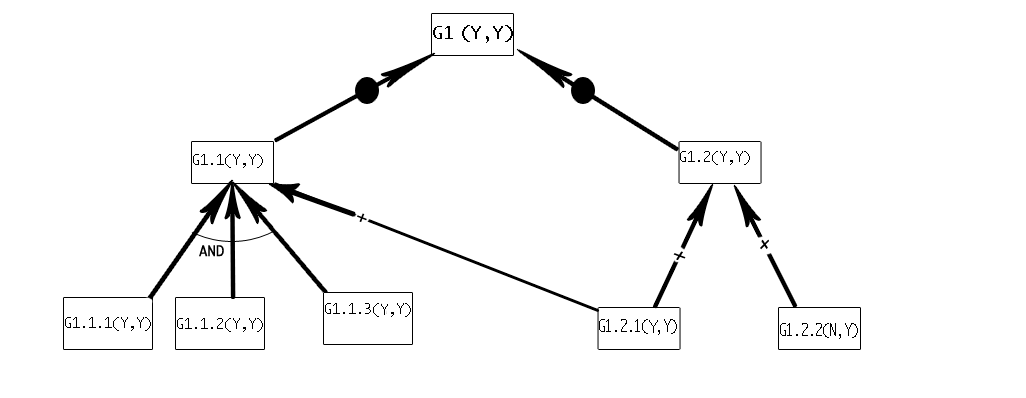
\includegraphics[width=3.4in]{img/5.PNG}
    \caption{SoF Annotated Goal Tree(Validated,Level 2 Elaboration)}
  \end{figure}
\end{frame}   

\begin{frame}  {Further Elaboration}   %[16]
  \begin{itemize}
  \item
    Here lists the detailed description of each goal that is not mentioned above.
    \begin{enumerate}
    \item $G_{1.1.1}$ is "Project managers input information of developers". 
    \item $G_{1.1.2}$ is "To access information of developers". 
    \item $G_{1.1.3}$ is "Project managers should update information of developers periodically". 
    \item $G_{1.1.1}$、$G_{1.1.2}$、$G_{1.1.3}$ work together to support their parent goal.
    \end{enumerate}
    If any of them fails to pass the evaluation, the whole elaboration plan fails.
  \end{itemize}
\end{frame}

\begin{frame} {Further Elaboration}
  \begin{itemize}
  \item
    \begin{enumerate}
    \item $G_{1.2.1}$ is "To provide an instant messaging platform for technical department managers, project managers and developers".
    \item  $G_{1.2.2}$ is "To publish decisions made by technical department managers and allow developers and project managers to reply asynchronously".
    \item $G_{1.2.1}$ does not conflict any other goal, and facilitates $G_{1.1}$ because the establishment of communication platform contributes positively to technical department managers' knowledge of developers' information. Thus $G_{1.2.1}$ passed both validations.
    \item $G_{1.2.2}$, although had passed the relevance validation, however, failed to pass the success validation because stakeholders believe that asynchronous communication is not practical and efficient enough to ensure the timeliness and richness of feedbacks.      
    \end{enumerate}
  \end{itemize}
\end{frame}

 

\section*{Summary}
\begin{frame}{Summary}
  \begin{itemize}
  \item
    Against requirements nondeterminism.%Acquire more complete and relevant requirements in practice of projects with requirements nondeterminism.
  \item
    Ensuring the quality of each step of elaboration.%The atomicity of SoF Elaboration Activity also ensures the quality of elaborations.
  \item 
    Consistency between goal models and stakeholders' conceptual models.%Each step of SoF activities is stakeholder-centered, which ensures that stakeholders' description of future system consists with goal models. With such consistency, SoF provides a reasonable context for KAOS Goal reasoning.
  \end{itemize}
  \vskip0pt plus.5fill
  \begin{itemize}
  \item
    Outlook
    \begin{itemize}
    \item
      Difficulty in validating the effectiveness of my proposal.
    \item
      Cost Problem.
      \begin{enumerate}
      \item considerably frequent communication between and among requirements developers and stakeholders %The development cost is relatively higher because recursively executing SoF Elaboration Activities requires considerably frequent communication between and among requirements developers and stakeholders, which will certainly result in unacceptably high cost under some circumstances.
      \item collection and management of raw data from stakeholders
      \item ubiquitous involvement of stakeholders %We should decide whether a project is adaptive in applying SoF methods at the beginning of each project. Some projects with relatively constant and determinate requirements are not supposed to apply SoF methods.
      \end{enumerate}
    \end{itemize}
  \end{itemize}
\end{frame}

\end{document}


